\documentclass{beamer}

\usetheme{shadow}
\usecolortheme{default}
% fine for B/W printing:
%\usecolortheme{seahorse}

%\usefonttheme{}
%\useinntertheme{}
%\useoutertheme{}

\usepackage{pgf,pgfarrows,pgfnodes,pgfautomata,pgfheaps,pgfshade}
\usepackage{graphicx}
\usepackage{epsfig}
\usepackage{fancyvrb,moreverb,relsize}
\usepackage{amsmath,amssymb}
\usepackage[latin1]{inputenc}
\usepackage{colortbl}
\usepackage[english]{babel}

% Use some nice templates
\beamertemplatetransparentcovereddynamic

% User's newcommands:
\newcommand{\emp}[1]{{\smaller\texttt{#1}}}
\newcommand{\mathbfx}[1]{{\mbox{\boldmath $#1$}}}

\begin{document}

\title{Beating the Limitations of Camera-Monitor Mediated Telepresence With Extra Eyes}

\author[author1 and author2]{author1\inst{1}
\and
author2\inst{2}}

\institute{MIT\inst{1}
\and
CMU\inst{2}}

\date{November 12, 2013}



% If you wish to uncover everything in a step-wise fashion, uncomment
% the following command: 

%\beamerdefaultoverlayspecification{<+->}

\begin{frame}
\titlepage
\end{frame}

\section[Abstract]{Abstract}


\begin{frame}
\frametitle{Abstract}

\begin{itemize}
\item In physical presence, you are most aware of your immediate surroundings, such as what is at your feet or who is beside you, and less aware of objects further away.
\item In telepresence, almost the opposite is true.
\item Due to the nature of the medium, you are most aware of what is in front, often at a distance, as dictated by the limited view of the camera.
\end{itemize}

\end{frame}

\begin{frame}
\frametitle{Abstract}

\begin{itemize}
\item Even where remote camera control is possible, the range of exploration is limited and the logistics of control are typically awkward and slow.
\item All of this adds up to a pronounced loss of awareness of the periphery in telepresence.
\item The research described here attempts to compensate for these problems through two mechanisms.
\end{itemize}

\end{frame}

\begin{frame}
\frametitle{Abstract}

\begin{itemize}
\item First, we provide telepresence users with two separate views, one wide-angle and the other, a controllable, detailed view.
\item To simplify navigation, the two views are seamlessly linked together, so that selecting a region of one will have an effect in the other.
\item Second, we utilize sensor information from the remote location to provide the user with notification of relevant events that may require attention.
\end{itemize}

\end{frame}

\section[Introduction]{Introduction}


\begin{frame}
\frametitle{Introduction}

\begin{itemize}
\item Normal human vision can be conceived as consisting of two highly mobile cones of view.
\item One is the focused foveal cone, one degree wide, while the second is the peripheral cone, or global field of view, spanning approximately 170 degrees .
\item Excellent spatial resolution is provided by the first, while the second, lower resolution view, provides us with stimulus that acts to redirect our attention.
\end{itemize}

\end{frame}

\begin{frame}
\frametitle{Introduction}

\begin{itemize}
\item Camera-monitor mediated vision, in contrast, suffers in resolution and due to the size of the display, uses limited azimuth of the visual field.
\item Watching television, for instance, typically involves the foveal cone only.
\end{itemize}

\end{frame}

\begin{frame}
\frametitle{Introduction}

\begin{itemize}
\item The narrow channel of information, both in the sense of bandwidth and field of view, imposes limitations on the ability to explore, follow conversations, check reactions, and generally sense significant actions in a remote space, such as people passing by or entering.
\item In such situations, users must choose between a global and a focused view.
\end{itemize}

\end{frame}

\begin{frame}
\frametitle{Introduction}

\begin{itemize}
\item With the former, resolution is sacrificed to permit a wide field of view and easy change of gaze direction.
\item If only the focused view is provided, users obtain details but no peripheral awareness.
\item This is typical of most videoconference settings  .
\item One approach to support both the foveal and peripheral cones is with multiple views.
\item The problems with this approach are well understood.
\end{itemize}

\end{frame}

\begin{frame}
\frametitle{Introduction}

\begin{itemize}
\item The Multiple Target Video (MTV) system of Gaver et. al.  first proposed the use of multiple cameras as a means of providing more flexible access to remote working environments.
\item Users were offered sequential access to several different views of a remote space.
\item However, as the authors noted, a static configuration of cameras will never be suitable for all tasks.
\end{itemize}

\end{frame}

\begin{frame}
\frametitle{Introduction}

\begin{itemize}
\item Furthermore, switching between views introduces confusing spatial discontinuities.
\item A further study (MTV II) by Heath et. al.  attempted to address this latter issue by providing several monitors, so that every camera view was simultaneously available.
\item While this new configuration was more flexible, the inability of static cameras to provide complete access to a remote space still remained a problem.
\end{itemize}

\end{frame}

\begin{frame}
\frametitle{Introduction}

\begin{itemize}
\item Furthermore, the various views were independent of one another, and the relationship between them was not made explicit.
\item Consequently, spatial discontinuities persisted.
\item Another approach involved the Virtual Window concept , which uses the video image of a person's head to navigate a motorized camera in a remote location.
\end{itemize}

\end{frame}

\begin{frame}
\frametitle{Introduction}

\begin{itemize}
\item Our user experience with this technique  revealed a significant improvement to the user's sense of engagement in meetings.
\item Unfortunately, when the camera was focused on a small area, the loss of global context often made the user unaware of important activity taking place out of view.
\item To compensate for the limitations on vision imposed by camera-monitor mediated telepresence, the work discussed here offers to:.
\end{itemize}

\end{frame}

\begin{frame}
\frametitle{Introduction}

\begin{itemize}
\item 1. Provide both a global (peripheral) and a detail (focused) view, simultaneously.
\item We note that this approach has already been used extensively in the Ontario Telepresence Project    by combining the two views through a picture-in-picture device.
\item The same approach with multiple views was also proposed by Kuzuoka et. al. .
\end{itemize}

\end{frame}

\begin{frame}
\frametitle{Introduction}

\begin{itemize}
\item However, as will be discussed later, providing a link between the two views is not only critical for usability, but also supports the goal of multiple views while avoiding the pitfalls of spatial discontinuities inherent in the MTV studies  .
\item 2. Provide a navigation mechanism using these views, allowing users to redirect their view in both direction and scale, through a simple user interface.
\end{itemize}

\end{frame}

\section[Supporting Foveal and Peripheral Cones]{Supporting Foveal and Peripheral Cones}


\begin{frame}
\frametitle{Supporting Foveal and Peripheral Cones}

\begin{itemize}
\item It has been suggested by several vision researchers that a brain mechanism exists to drive foveating saccades of the eye in response to stimulus in the periphery region  .
\item In the discussion of their model of saccadic eye movement, Tsotsos et al. comment that these saccades play an important role in the exploration of the visual world .
\item Supporting evidence for this comes from neurophysiology.
\end{itemize}

\end{frame}

\begin{frame}
\frametitle{Supporting Foveal and Peripheral Cones}

\begin{itemize}
\item A region known as PO, which receives a representation of the periphery of the visual field, has been identified in the brains of primates .
\item Deprived of this information, individuals suffering from tunnel vision, or a loss of vision outside the fovea, exhibit severe problems navigating through their physical surroundings, even when these surroundings are familiar to them .
\end{itemize}

\end{frame}

\begin{frame}
\frametitle{Overlaid Multiple Views}

\begin{itemize}
\item As an initial attempt to provide this support, we developed a prototype system, consisting of a large and small display, as shown in Figure 1.
\item The large screen display provides the user with a wide angle view of the remote space while the small display provides a high resolution view of the area of interest.
\item With the camera orientations fixed and the proper geometric positioning of the two displays, spatial discontinuities are minimized.
\end{itemize}

\end{frame}

\begin{frame}
\frametitle{Overlaid Multiple Views}

\begin{itemize}
\item The sensation of increased peripheral awareness obtained by this system is very powerful.
\item We note that this prototype requires two high-resolution displays, one of them quite large, in order to achieve a significant effect.
\item As this may be prohibitively expensive for most videoconference users, we would like to unify the two views into a single display.
\end{itemize}

\end{frame}

\begin{frame}
\frametitle{}


\begin{columns}

\column{1\textwidth}
\centerline{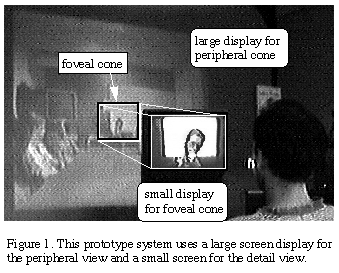
\includegraphics[width=0.500000\linewidth,keepaspectratio]{ky_fg1.png}}

\end{columns}

\end{frame}

\begin{frame}
\frametitle{Disjointed Multiple Views}

\begin{itemize}
\item Another approach to supporting both the foveal and peripheral views is to display the two separately on the same screen.
\item Since the views are disjointed, each can have sufficient size and resolution, even with the limitations of current technology.
\item Our implementation of this system is shown in Figure 2.
\end{itemize}

\end{frame}

\begin{frame}
\frametitle{Disjointed Multiple Views}

\begin{itemize}
\item The top portion of the display provides a foveal or detail view, obtained from a user-controlled motorized camera, while the lower portion provides the peripheral or global view from a fixed, wide-angle camera.
\item Since the views are independent of each another, there is no consistent geometric relationship between the two.
\end{itemize}

\end{frame}

\begin{frame}
\frametitle{Disjointed Multiple Views}

\begin{itemize}
\item This can result in an inability to locate the position of the detailed region within the peripheral view, once more bringing us back to the problem of spatial discontinuities.
\item Navigation under these conditions is typically difficult and slow.
\item This is especially severe when the scene being viewed is relatively homogeneous (e.g. through tele-education, a large class of students).
\end{itemize}

\end{frame}

\begin{frame}
\frametitle{}


\begin{columns}

\column{1\textwidth}
\centerline{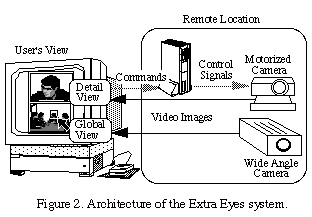
\includegraphics[width=0.500000\linewidth,keepaspectratio]{ky_fg2.png}}

\end{columns}

\end{frame}

\begin{frame}
\frametitle{Linking Multiple Views}

\begin{itemize}
\item To address the lack of a geometric relationship between the two views, we indicate the detailed region within the global view by means of a yellow bounding box (detail frame), as shown in Figure 3.
\item The enclosed region corresponds exactly to what is displayed in the detail view.
\item As the detail view changes, the bounding box on the global view adjusts accordingly.
\end{itemize}

\end{frame}

\begin{frame}
\frametitle{Linking Multiple Views}

\begin{itemize}
\item Because the two views are logically linked, users can select a desired region by sweeping out a bounding box or simply point-and-click on the global view.
\item In the former case, the detail view is defined by the size of the bounding box, while in the latter, the detail view is centered at the selected position and displayed at the maximum zoom.
\end{itemize}

\end{frame}

\begin{frame}
\frametitle{Linking Multiple Views}

\begin{itemize}
\item These interaction techniques with the global view permit a far more efficient navigation mechanism than the effectively blind view selection offered by both the original MTV system  and the Virtual Window system .
\item In addition to control via the global view, the detail view can be manipulated directly through the scroll bars, which provide tilt and pan control of the motorized camera.
\end{itemize}

\end{frame}

\begin{frame}
\frametitle{Linking Multiple Views}

\begin{itemize}
\item It is also possible to adjust the zoom factor of the detail view by pressing the left or right mouse button, or obtain a wide view by selecting the wide button.
\item To provide a linkage between the global and detail views, we require a mapping between the coordinate systems of each, dependent on the properties of the different cameras.
\item We first define a global coordinate system, which covers the entire area visible to both cameras.
\end{itemize}

\end{frame}

\begin{frame}
\frametitle{Linking Multiple Views}

\begin{itemize}
\item Next, we define models for each camera, which consist of a view model, and in the case of the motorized camera, a transformation function.
\item The models describe the relationship between pixel coordinates of each camera and the global coordinate system.
\item In the case of our fixed wide-angle camera, this is simply a one-to-one mapping.
\item The transformation function for the motorized camera maps pixel coordinates to the appropriate motor signals.
\end{itemize}

\end{frame}

\begin{frame}
\frametitle{Linking Multiple Views}

\begin{itemize}
\item The models and relationships are described in Figure 4.
\item When a user selects an area of the global view, the pixel coordinates of this region are first translated into global coordinates through the wide angle view model, and then into pixel coordinates of the detail view.
\item The detail pixel coordinates are then mapped into motor signals via the transformation function.
\item Finally, the motor signals are sent to the detail camera.
\end{itemize}

\end{frame}

\begin{frame}
\frametitle{}


\begin{columns}

\column{1\textwidth}
\centerline{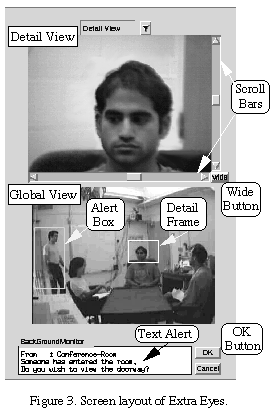
\includegraphics[width=0.500000\linewidth,keepaspectratio]{ky_fg3.png}}

\end{columns}

\end{frame}

\begin{frame}
\frametitle{}


\begin{columns}

\column{1\textwidth}
\centerline{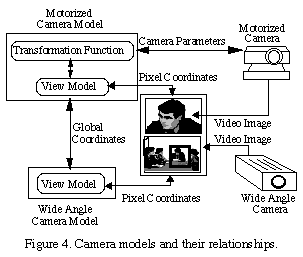
\includegraphics[width=0.500000\linewidth,keepaspectratio]{ky_fg4.png}}

\end{columns}

\end{frame}

\section[Sensory Surrogate]{Sensory Surrogate}


\begin{frame}
\frametitle{Sensory Surrogate for Environmental Awareness}

\begin{itemize}
\item There exists no substitute for physical presence that offers the fidelity of rapidly directable stereo vision and spatially sensitive binaural audio, as manifested by the human senses.
\item To help bridge the gap between physical presence and telepresence in this regard, our Extra Eyes system provides users with a sensory surrogate to increase their awareness of the remote environment.
\end{itemize}

\end{frame}

\begin{frame}
\frametitle{Sensory Surrogate for Environmental Awareness}

\begin{itemize}
\item The surrogate monitors background information obtained by sensors and reports on relevant events through the use of sound, text, and graphics, or a combination of the three.
\item In this manner, background processing by the computer is used to improve the user's foreground awareness.
\end{itemize}

\end{frame}

\begin{frame}
\frametitle{Sensory Surrogate for Environmental Awareness}

\begin{itemize}
\item Sensors in the room  monitor the status of presentation technology such as the VCR, document camera, and digital whiteboard, as well as the entry of new individuals as depicted in Figure 5.
\item When an event occurs, it triggers an alert-action sequence.
\end{itemize}

\end{frame}

\begin{frame}
\frametitle{Sensory Surrogate for Environmental Awareness}

\begin{itemize}
\item The alert corresponds to the screen message displayed (e.g. "Someone has entered the room. Do you wish to view the doorway?"), as well as the appearance of a blue bounding box (alert box) in the corresponding region of the global view, as shown in Figure 3.
\end{itemize}

\end{frame}

\begin{frame}
\frametitle{}


\begin{columns}

\column{1\textwidth}
\centerline{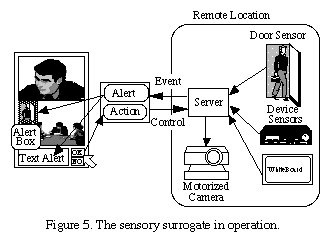
\includegraphics[width=0.500000\linewidth,keepaspectratio]{ky_fg5.png}}

\end{columns}

\end{frame}

\begin{frame}
\frametitle{}


\begin{columns}

\column{1\textwidth}
\centerline{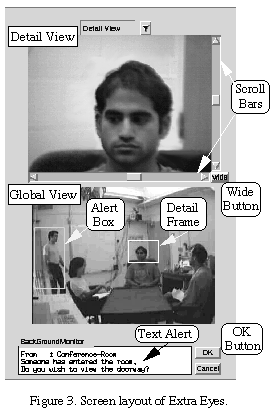
\includegraphics[width=0.500000\linewidth,keepaspectratio]{ky_fg3.png}}

\end{columns}

\end{frame}

\begin{frame}
\frametitle{Sensory Surrogate for Social Awareness}

\begin{itemize}
\item We have also applied the sensory surrogate concept to increasing social awareness among individuals sharing the media space of the Ontario Telepresence Project .
\item The Postcards system (see Figure 6), based on Rank Xerox EuroPARC's Portholes , captures snapshots from each user's office at set intervals and distributes these to members of the media space.
\end{itemize}

\end{frame}

\begin{frame}
\frametitle{Sensory Surrogate for Social Awareness}

\begin{itemize}
\item A sensory surrogate in the Postcards system compares every two consecutive frames from each office to determine if there is activity there.
\item This is done by counting the number of pixels that have changed by more than a certain threshold amount between the two frames.
\item Although the algorithm is susceptible to false detection of activity due to camera perturbations, it has worked reasonably well in our environment.
\end{itemize}

\end{frame}

\begin{frame}
\frametitle{Sensory Surrogate for Social Awareness}

\begin{itemize}
\item Stored knowledge of activity allows Postcards to determine whether individuals are in or out, or have recently entered or vacated their offices.
\item Users can take advantage of this background monitoring feature by asking the system to sense activity and notify them when any number of individuals are simultaneously present in their offices.
\end{itemize}

\end{frame}

\begin{frame}
\frametitle{}


\begin{columns}

\column{1\textwidth}
\centerline{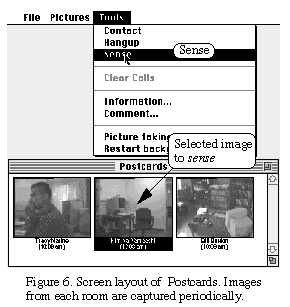
\includegraphics[width=0.500000\linewidth,keepaspectratio]{ky_fg6.png}}

\end{columns}

\end{frame}

\section[Evaluation]{Evaluation}


\begin{frame}
\frametitle{User Study}

\begin{itemize}
\item We evaluated the performance of Extra Eyes through the following user study.
\item Three television monitors were arranged in a remote location, as shown in Figure 7.
\item Letters of the alphabet were displayed on a randomly chosen monitor, one at a time.
\item The user's task was to use the Extra Eyes system to identify these letters as they appeared, as quickly as possible, while minimizing the number of errors.
\end{itemize}

\end{frame}

\begin{frame}
\frametitle{User Study}

\begin{itemize}
\item Each letter would remain on the monitor until the user had identified it, by typing its corresponding key.
\item Once the letter was identified, it would be replaced by another letter on a different monitor.
\item The font size was sufficiently small so that a zoom factor near the maximum was required for legibility.
\item We tested each of our seven subjects on the following conditions, the order being randomly varied, with 20 repetitions per condition:.
\end{itemize}

\end{frame}

\begin{frame}
\frametitle{User Study}

\begin{itemize}
\item 1. No Global: Only the detail view is visible.
\item This situation is equivalent to typical telepresence systems.
\item 2. No Global + Text: Same as 1.
\item In addition, a text alert indicates the display on which the current letter appears.
\item 3. Unlinked: Both the global and detail views are simultaneously visible, but the two views are not linked (i.e. neither view has effect on the other).
\item This is equivalent to the MTV system.
\end{itemize}

\end{frame}

\begin{frame}
\frametitle{User Study}

\begin{itemize}
\item 4. Linked: Both the global and detail views are simultaneously visible and linked.
\item 5. Linked + Text: Same as 4.
\item In addition, a text alert indicates the display on which the current letter appears.
\item 6. Linked + Action: Same as 5.
\item In addition, an alert box appears, and the user can invoke the action corresponding to the alert by pushing the OK button or by clicking anywhere within the alert box.
\end{itemize}

\end{frame}

\begin{frame}
\frametitle{}


\begin{columns}

\column{1\textwidth}
\centerline{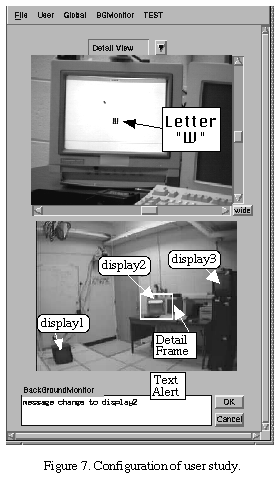
\includegraphics[width=0.500000\linewidth,keepaspectratio]{ky_fg7.png}}

\end{columns}

\end{frame}

\begin{frame}
\frametitle{Discussion and Results of User Study}

\begin{itemize}
\item For the first three conditions, users exhibited two strategies to identify the various letters.
\item When no information beyond that of the detail view was available, users consistently zoomed out to obtain a wide angle view, then panned and tilted the camera to center the letter, before zooming in again.
\end{itemize}

\end{frame}

\begin{frame}
\frametitle{Discussion and Results of User Study}

\begin{itemize}
\item This zoom-out strategy, represented by the solid line in the space-scale diagram  of Figure 8a, requires over three camera operations, on average, to identify each letter.
\item When an alert message was added, indicating the display on which the new letter appears, users tended to change their strategy.
\end{itemize}

\end{frame}

\begin{frame}
\frametitle{Discussion and Results of User Study}

\begin{itemize}
\item Knowing the approximate location of the desired monitor from past experience gathered during the study, users often tried to find this monitor by repeatedly panning and tilting the camera, as shown by the solid line in Figure 8b.
\item This strategy is quite similar to searching for an object in a familiar room, while in the dark.
\end{itemize}

\end{frame}

\begin{frame}
\frametitle{Discussion and Results of User Study}

\begin{itemize}
\item Because users cannot accurately select a desired position with the pan-tilt strategy, this method often requires more operations than the zoom-out strategy.
\item The same pan-tilt strategy was used when the global view was provided, but not linked to the detail view.
\item For the remaining three conditions, users were able to identify the letters with only a single camera operation.
\end{itemize}

\end{frame}

\begin{frame}
\frametitle{Discussion and Results of User Study}

\begin{itemize}
\item Figure 9 and Figure 10 present the results of our user study, indicating the average number of camera operations users required to identify each letter, as well as the average completion time with 95\% confidence error bars, with each of the six experimental conditions.
\item Analysis of variance (ANOVA) showed that both number of operations and trial completion times were significantly affected by the experimental conditions.
\end{itemize}

\end{frame}

\begin{frame}
\frametitle{Discussion and Results of User Study}

\begin{itemize}
\item For number of operations, F(5, 30)=55.2, p<0.001.
\item For completion time, F(5, 30)=40.1, p<0.001.
\item As measured by number of operations (Table A1 in the Appendix), Fisher's protected LSD posthoc analyses showed that all linked conditions were significantly different from the Unlinked and NoGlobal conditions (p<0.05).
\item However, there is no significant difference among linked conditions.
\end{itemize}

\end{frame}

\begin{frame}
\frametitle{Discussion and Results of User Study}

\begin{itemize}
\item The difference between Unlinked and NoGlobal, as well as Unlinked and NoGlobal+Text is also insignificant.
\item As measured by completion times (Table A2 in the Appendix), Fisher's protected LSD posthoc analyses showed that all conditions were significantly different from each other (p<0.05), except Linked+Action vs. Linked+Text condition (p=0.64) and NoGlobal vs. Unlinked (p=0.66).
\end{itemize}

\end{frame}

\begin{frame}
\frametitle{}


\begin{columns}

\column{1\textwidth}
\centerline{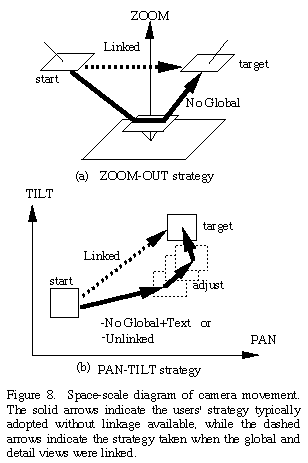
\includegraphics[width=0.500000\linewidth,keepaspectratio]{ky_fg8.png}}

\end{columns}

\end{frame}

\begin{frame}
\frametitle{}


\begin{columns}

\column{1\textwidth}
\centerline{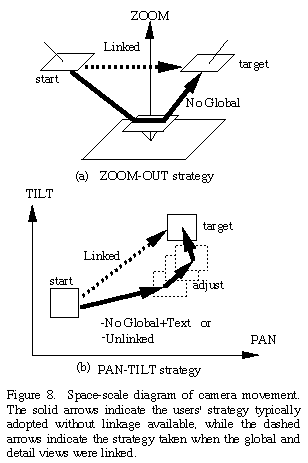
\includegraphics[width=0.500000\linewidth,keepaspectratio]{ky_fg8.png}}

\end{columns}

\end{frame}

\begin{frame}
\frametitle{}


\begin{columns}

\column{1\textwidth}
\centerline{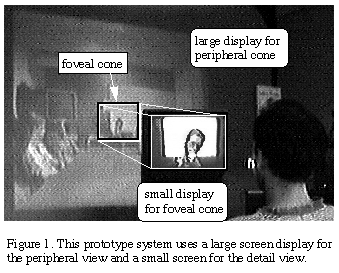
\includegraphics[width=0.500000\linewidth,keepaspectratio]{ky_fg1.png}}

\end{columns}

\end{frame}

\begin{frame}
\frametitle{}


\begin{columns}

\column{1\textwidth}
\centerline{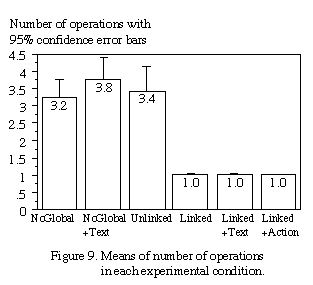
\includegraphics[width=0.500000\linewidth,keepaspectratio]{ky_fg9.png}}

\end{columns}

\end{frame}

\begin{frame}
\frametitle{Figure 9 and Figure 10 present the results of our user study, indicating the average number of camera operations users required to identify each letter, as well as the average completion time with 95\% confidence error bars, with each of the six experimental conditions.}


\begin{columns}

\column{1\textwidth}
\centerline{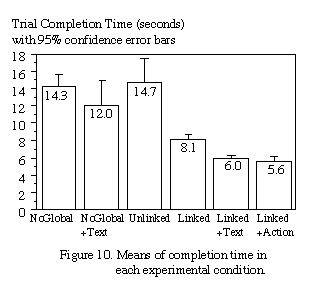
\includegraphics[width=0.500000\linewidth,keepaspectratio]{ky_fg10.png}}

\end{columns}

\end{frame}

\begin{frame}
\frametitle{}


\begin{columns}

\column{1\textwidth}
\centerline{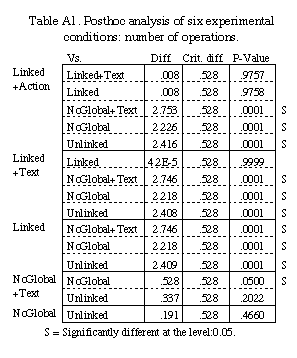
\includegraphics[width=0.500000\linewidth,keepaspectratio]{ky_fg11.png}}

\end{columns}

\end{frame}

\begin{frame}
\frametitle{}


\begin{columns}

\column{1\textwidth}
\centerline{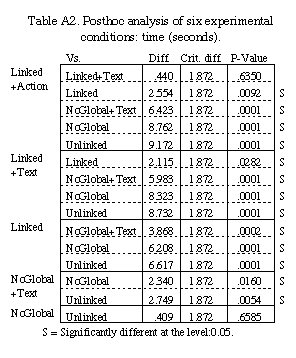
\includegraphics[width=0.500000\linewidth,keepaspectratio]{ky_fg12.png}}

\end{columns}

\end{frame}

\begin{frame}
\frametitle{Conclusion 1: Linkage Between Views is Very Important}

\begin{itemize}
\item When the two views were linked, navigation in the remote environment via selection in the global view was effortless.
\item Any desired (visible) target could be selected directly with a single camera operation, as indicated by the dashed lines of Figures 8a and 8b (see also Figure 9).
\item In this case, the previous indirect strategies of zoom-out and pan-tilt, which require almost twice as much time as direct selection, were never used.
\end{itemize}

\end{frame}

\begin{frame}
\frametitle{Conclusion 1: Linkage Between Views is Very Important}

\begin{itemize}
\item Users expressed their opinion that the direct selection mechanism was more natural than the indirect methods.
\item Indeed, all linked conditions were significantly better than the unlinked one in terms of both number of operations and trial completion time.
\item Further user feedback was also highly informative.
\item Some commented that the detail frame was useful as an indication of direction of camera motion.
\end{itemize}

\end{frame}

\begin{frame}
\frametitle{}


\begin{columns}

\column{1\textwidth}
\centerline{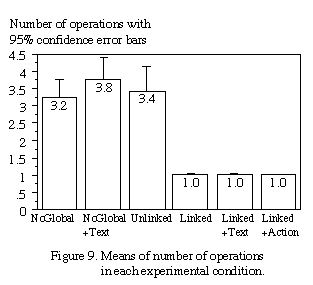
\includegraphics[width=0.500000\linewidth,keepaspectratio]{ky_fg9.png}}

\end{columns}

\end{frame}

\begin{frame}
\frametitle{Conclusion 2: Sensory Information is Useful}

\begin{itemize}
\item The time improvement from linked views to linked views with a text alert (p<0.05, see Table A2) indicates the added value of sensory information.
\item As most users explained, the alert allowed them to reduce the size of the visual search area.
\item Users also appreciated the audio feedback of a beep, provided simultaneously with an alert message, indicating that a new letter was about to appear.
\end{itemize}

\end{frame}

\begin{frame}
\frametitle{Conclusion 2: Sensory Information is Useful}

\begin{itemize}
\item We note that sensory information may have compensated for the low update rate (approximately 1-2 frames/s in our present implementation) of the global view.
\item In many instances, the indication of various alerts preceded the appearance of a new letter on the global view by one second or more.
\item This enabled users to begin their navigation toward the desired monitor before the letter was actually visible.
\end{itemize}

\end{frame}

\begin{frame}
\frametitle{Conclusion 2: Sensory Information is Useful}

\begin{itemize}
\item Although the differences in time and number of operations between Linked+Text and Linked+Action were not statistically significant, users indicated that the graphic alerts were more useful than text messages.
\item The graphic alerts completely specify the relevant visual regions, as opposed to text alerts, which require the user to read and then perform a search.
\end{itemize}

\end{frame}

\begin{frame}
\frametitle{}


\begin{columns}

\column{1\textwidth}
\centerline{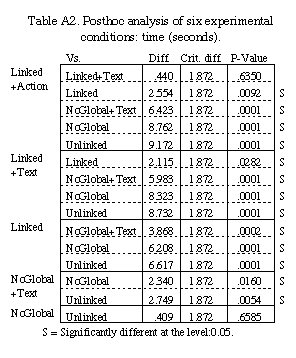
\includegraphics[width=0.500000\linewidth,keepaspectratio]{ky_fg12.png}}

\end{columns}

\end{frame}

\section[Further Issues]{Further Issues}


\begin{frame}
\frametitle{Further Issues}

\begin{itemize}
\item Having described Extra Eyes and our preliminary evaluation of this system, we now turn to some other issues.
\item The global view provided by our present system can not capture a view of the entire room.
\item Other designers may prefer to use multiple cameras, or a very wide angle lens, possibly a fisheye, for this task.
\end{itemize}

\end{frame}

\begin{frame}
\frametitle{Further Issues}

\begin{itemize}
\item In the former case, some form of image processing will be required to combine the images, while in the latter, unwarping to compensate for image distortion will be necessary.
\item Detractors may argue that transmitting video for the global view is too expensive.
\item Either more bandwidth is required, or the frame rate of the detail view will suffer.
\end{itemize}

\end{frame}

\begin{frame}
\frametitle{Further Issues}

\begin{itemize}
\item We suggest that since the global view is only required to provide a sense of peripheral awareness, both its frame rate and resolution can be relatively low.
\item In fact, we reduced our global view to a quarter size (160 x 120 pixels), and found that users were still very aware of activities occurring in the periphery.
\end{itemize}

\end{frame}

\section[Future Work]{Future Work}


\begin{frame}
\frametitle{Future Work}

\begin{itemize}
\item While the sense of peripheral awareness offered by a fixed global view is a helpful navigation tool, it does not accurately replicate the mechanics of human vision, in which the periphery is dictated by the orientation of the fovea.
\end{itemize}

\end{frame}

\begin{frame}
\frametitle{Future Work}

\begin{itemize}
\item A future version of Extra Eyes should remedy this shortcoming, either by attaching the global camera to the motorized detail camera, or by using another motorized camera for the global view, synchronized with the detail camera.
\item This improvement is presently being applied to our initial large-screen prototype, discussed earlier.
\item To maximize effectiveness, we are locating the smaller display near the center of the large screen.
\end{itemize}

\end{frame}

\begin{frame}
\frametitle{Future Work}

\begin{itemize}
\item This way, the foveal and peripheral cones will maintain the correct geometric relationship at all times.
\item We are presently combining such a system with the Virtual Window head-tracking mechanism, and look forward to reporting on its results in the near future.
\end{itemize}

\end{frame}

\section[Conclusions]{Conclusions}


\begin{frame}
\frametitle{Conclusions}

\begin{itemize}
\item We have crossed the complexity barrier of current camera-monitor mediated telepresence applications.
\item To beat the limitations imposed by this barrier, we propose a new design to support views of the foveal and peripheral cones simultaneously.
\item To minimize the effects of spatial discontinuities, we also provide a seamless linkage between the two views.
\end{itemize}

\end{frame}

\section[Acknowledgments]{Acknowledgments}


\begin{frame}
\frametitle{Acknowledgments}

\begin{itemize}
\item The authors would like to thank William Hunt and Shumin Zhai of the University of Toronto, Abigail Sellen of Rank Xerox EuroPARC and Masayuki Tani of Hitachi Research Laboratory, for their invaluable suggestions and contributions to this paper.
\item We would also like to thank John Tsotsos of the University of Toronto for helping us sift through the relevant literature on biological vision.
\end{itemize}

\end{frame}

\begin{frame}
\frametitle{Acknowledgments}

\begin{itemize}
\item This research has been undertaken as part of the Ontario Telepresence Project.
\end{itemize}

\end{frame}

\section[Appendix]{Appendix}


\end{document}
